\begin{frame}{Bosonic Mott Insulators}
\vskip-1.5cm

\only<1>{
        \begin{figure}
        \centering
        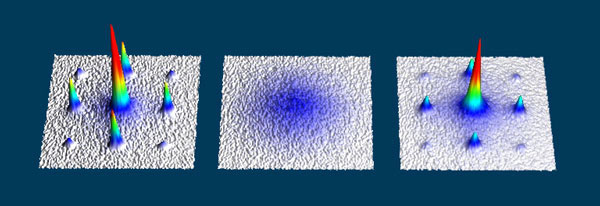
\includegraphics[width=\linewidth]{diagrams/SuperfluidStates.jpg}
        \caption{Mott insulator with cold atoms in optical lattice\footnotemark}
        \end{figure}
        }
\begin{block}{Bose-Hubbard model}
\vskip-0.3cm
$$
H_{BH} = -J \sum\limits_{<ij>} b^{\dagger}_i b_j - \mu \sum\limits_i N_i + \frac12 V \sum\limits_i N_i (N_i-1)
$$
\end{block}
\only<2->{
\begin{columns}[T]
    \begin{column}[T]{.4\textwidth}
        \vskip-1.2cm

        \only<2>{
        \begin{figure}
        \centering
        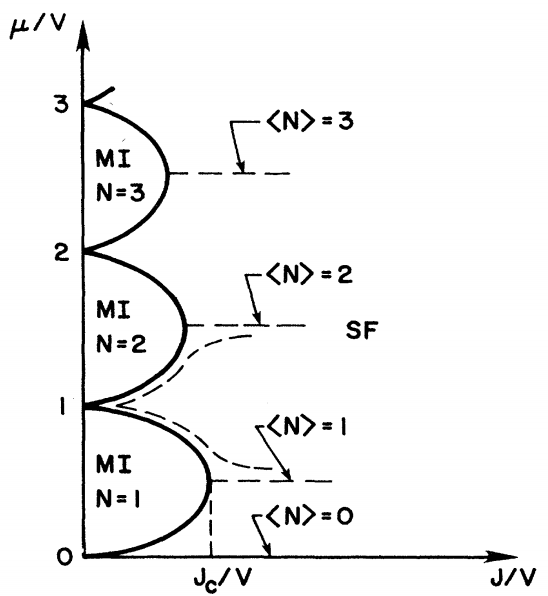
\includegraphics[width=\linewidth]{diagrams/bosehubbard2.png}
        \end{figure}
        }
    \end{column}
    \begin{column}[T]{.6\textwidth}
    \vskip-0.7cm
    \bi
    \item Form an atomic insulator with N bosons to minimize $-\mu N + VN(N-1)/2$
    %Particles and holes have a cost based on this function
    %particle cost goes to zero at transition between fillings
    \item Gap to particle/hole excitations
    %Kinetic energy causes some local density fluctuations, but not much else
    \item Bosons free to hop will instantly condense into superfluid with any $J$
    %Must have interactions, and in cold atoms
    %Deep optical lattice wells to keep $J$ small enough
    \item Number conserving - so no superfluid phase coherence
    %\item Unlike free-fermions, not obvious how to construct fractional site filling insulators
    %\item Tensor network states give us access to needed construction and to interacting invariants.
    %\note{LSM inspired invariants}
    \ei
    \end{column}
\end{columns}
}
\only<1>{
\footnotetext[3]{\citep{Greiner2002-ay}}
}
\only<2>{
\footnotetext[4]{\citep{Fisher1989-ou}}
}
\end{frame}
